\documentclass{article}
\usepackage[utf8]{inputenc}
\usepackage{amsmath}
\usepackage{amssymb}
\usepackage{natbib}
\usepackage{graphicx}
\usepackage{listings}
\usepackage{color}
\usepackage{tikz}
\usepackage{multicol}
\usetikzlibrary{arrows}
\usepackage{hyperref}
\hypersetup{
    colorlinks=true,
    linkcolor=blue,
    filecolor=magenta,      
    urlcolor=cyan,
}
\usepackage{float}
\restylefloat{figure}

%\usepackage[figurename=Figur]{caption}

\newcommand{\pd}[2]{\frac{\partial #1}{\partial #2}}

\definecolor{codegreen}{rgb}{0,0.6,0}
\definecolor{codegray}{rgb}{0.5,0.5,0.5}
\definecolor{codepurple}{rgb}{0.58,0,0.82}
\definecolor{backcolour}{rgb}{0.95,0.95,0.92}
 
\lstdefinestyle{mystyle}{
    backgroundcolor=\color{backcolour},   
    commentstyle=\color{codegreen},
    keywordstyle=\color{magenta},
    numberstyle=\tiny\color{codegray},
    stringstyle=\color{codepurple},
    basicstyle=\footnotesize,
    breakatwhitespace=false,         
    breaklines=true,                 
    captionpos=b,                    
    keepspaces=true,                 
    numbers=left,                    
    numbersep=5pt,                  
    showspaces=false,                
    showstringspaces=false,
    showtabs=false,                  
    tabsize=2
}
 
\lstset{style=mystyle}
\lstset{
    language=Erlang,
    mathescape=true
}

\title{Oblig 3}
\author{Hans-Petter Harveg}
\date{November 10th, 2017}

\begin{document}
\maketitle

\section*{Project 1}

\subsection*{a.}

I have two solutions to this one, so I will include both

\subsubsection*{1. Using the var der Walls equation and simply solve for $P$}

\begin{equation}
(p + \frac{aN^2}{V^2})(V - Nb) = NkT \rightarrow p = \frac{NkT}{V-Nb} - \frac{aN^2}{V^2}
\end{equation}

\subsubsection*{2. Taking the derivative of $F_{vdW}$, with respect to $V$}

\begin{align*}
p & = -\frac{\partial F_{vdW}}{\partial V} = -\frac{\partial}{\partial V}\bigg[-NkT(\ln \bigg( \frac{n_q(V-Nb)}{N} \bigg) + 1) - \frac{aN^2}{V} \bigg]\\
 & = -(-NkT\bigg(\frac{1}{V-Nb}\bigg) + \frac{aN^2}{V^2})\\
 & = NkT\bigg(\frac{1}{V-Nb}\bigg) - \frac{aN^2}{V^2}
\end{align*}

\begin{equation}
 p = NkT\bigg(\frac{1}{V-Nb}\bigg) - \frac{aN^2}{V^2}
\end{equation}

\subsection*{b.}

Introducing the following sizes

\begin{equation*}
p_c = \frac{a}{27b^2} \ \ , \ \ V_c = 3Nb \ \ , \ \ kT_c = \frac{8a}{27b}
\end{equation*}

\begin{equation*}
\hat{p} = \frac{p}{p_c} \ \ , \ \ \hat{V} = \frac{V}{V_c} \ \ , \ \ \hat{T} = \frac{T}{T_c}
\end{equation*}


We can write $(eq.2)$ as

\begin{equation*}
\hat{p}p_c = \frac{Nk\hat{T}T_c}{\hat{V}V_c - Nb} - \frac{aN^2}{(\hat{V}V_c)^2}
\end{equation*}

\begin{equation*}
\hat{p}\bigg(\frac{a}{27b^2}\bigg) = \frac{Nk\hat{T}\bigg(\frac{8a}{27b}\bigg)}{\hat{V}(3Nb) - Nb} - \frac{aN^2}{(\hat{V}(3Nb))^2}
\end{equation*}

\begin{equation}
\rightarrow \hat{p} = \frac{8\hat{T}}{3\hat{V} - 1} - \frac{3}{\hat{V}^2}
\end{equation}


\subsection*{c.}

The script can be found \hyperlink{code_problem_c}{here}

\begin{figure}[H]
    \centering
    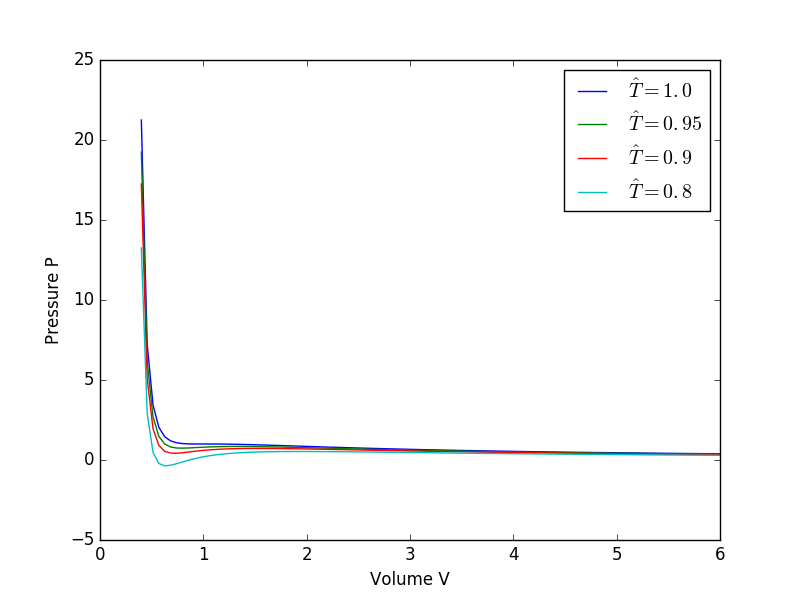
\includegraphics[width=4in]{project_1/problem_c}
    \caption[Plot from problem c.]
    {The pressure $\hat{P}$ as a function of $\hat{V}$ for $\hat{V}$ = $[0.4:6.0]$ for $\hat{T} = [1.0, 0.95, 0.9,0.08]$}
\end{figure}


\subsection*{d.}

Introducing the following sizes

\begin{equation}
\hat{\rho} = \frac{1}{\hat{V}} = \frac{\rho}{\rho_c} \ \ , \ \ \rho_c = \frac{1}{3b} \rightarrow \hat{V} = \frac{\rho_c}{\rho} = \frac{1}{\rho 3b}
\end{equation}

Using $(eq. 2)$, we can write the dimensionless equation

\begin{align*}
\hat{\rho} & = \frac{8\hat{T}}{3\hat{V} - 1} - \frac{3}{\hat{V}^2}\\
           & = \frac{8\hat{T}}{3\big(\frac{1}{\rho 3b}\big)-1} - \frac{3}{\big(\frac{1}{\rho 3b}\big)^2}\\
           & = \frac{8\hat{T}}{3\big(\frac{1}{\rho 3b} - 1\big)} - \frac{3}{\big(\frac{1}{\hat{\rho}}\big)^2}\\
           & = \frac{8\hat{T}}{\frac{3 - \hat{\rho}}{\hat{\rho}}} - 3\hat{\rho}^2
\end{align*}

\begin{equation}
\rightarrow \frac{8\hat{T}\hat{\rho}}{3 - \hat{\rho}} - 3\hat{\rho}^2
\label{eq:dimlessPress_vol}
\end{equation}

\subsection*{e.}

The script can be found \hyperlink{code_problem_e}{here}

\begin{figure}[H]
    \centering
    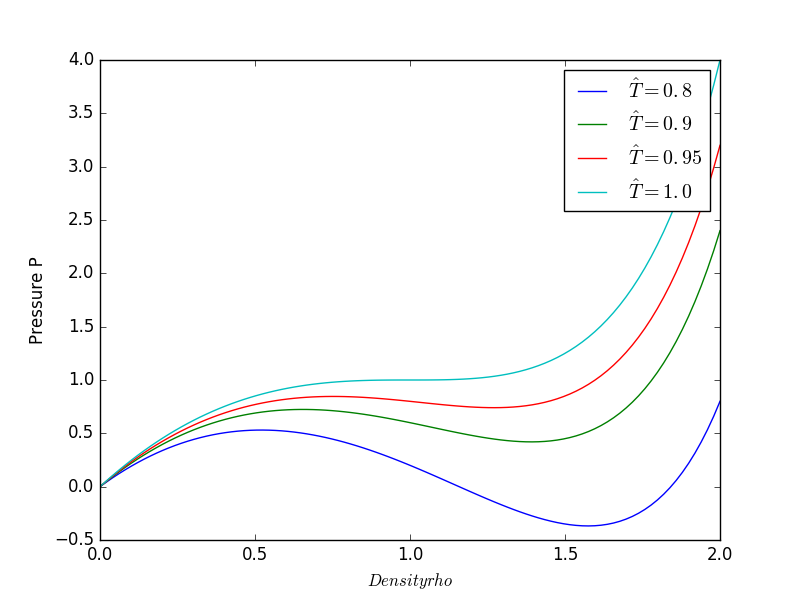
\includegraphics[width=4in]{project_1/problem_e}
    \caption[Plot from problem e.]
    {The pressure $\hat{P}$ as a function of $\hat{\rho}$ for $\hat{\rho}$ = $[0.0:2.0]$ for $\hat{T} = [0.8, 0.9, 0.95,1.0]$}
\end{figure}


\subsection*{f.}

  We can see from the plot that for the temperature $T = 1.0$, the density is an unique function, while for temperatures $T<1.0$, the density become non-uniqe. Meaning we can observe several similar densities for a given temperature for temperatures below $1.0$.

\subsection*{g.}

  We want to see where the isothermal compressibility is negative. The isothermal compressibility is defined as

\begin{equation}
\kappa = \frac{1}{\rho}\bigg(\frac{\partial\rho}{\partial P}\bigg)
\end{equation}

  We can see from the plot that for $T = 1.0$, the isothermal compressibility stay possitive. It seems to flatten out around $\rho \approx 0.8$, then, around $\rho \approx 1.2$, it increases again.

  For temeratures $T < 1.0$, we can see that the isothermal compressibility becomes negative around $\rho = 0.5 \approx 0.8$, depending on the temperature, and return to possitive around $\rho = 1.2 \approx 1.7$, depending on the temperature.

TODO: WHY IS NEGATIVE COMPRESSIBILITY A NON-PHYSICAL CONDITION?


\subsection*{h.}

We will now look at the PV isotherms of $N_2$. Using \eqref{eq:dimlessPress_vol}, we can write the equation as

\begin{equation}
P = P_c\left[\frac{\hat{8T/T_c}}{3\hat{V}/V_c - 1} - \frac{3V_c^2}{\hat{V}^2}\right]
\end{equation}

Where

\begin{equation}
P_c = 33.6 \text{ atm}, \qquad V_c = 0.089 \text{ l/mol}, \qquad T_c = 126 \text{ K}
\end{equation}

The script can be found \hyperlink{code_problem_h}{here}

\begin{figure}[H]
    \centering
    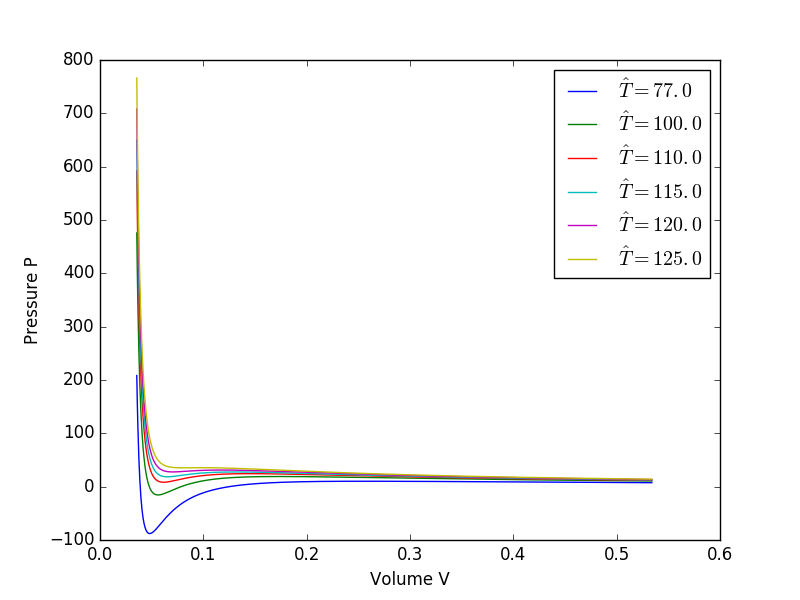
\includegraphics[width=4in]{project_1/problem_h}
    \caption[Plot from problem h.]
    {To relate the van der Waals fluid to nitrogen $(N_2)$ gas, we have used the numerical values for the sizes from problem \textbf{b.}; $p_c = 33.6 atm$, $V_c = 0.089 1/mol$ and $T_c = 126 K$ to plot, using the var der Waals equation of state the $PV$ isoterms of $N_2$ for $\hat{T} = [77K, 100K, 110K, 115K, 125K]$}
\end{figure}


\subsection*{i.}

We can find the equal area by drawing a straing line using "bye eye" appriximation. 

The script can be found \hyperlink{code_problem_i}{here}

\begin{figure}[H]
    \centering
    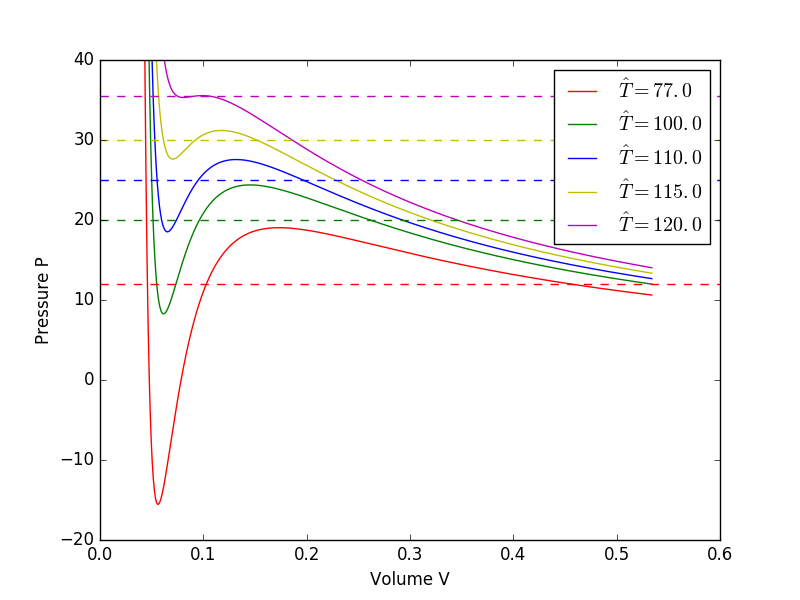
\includegraphics[width=4in]{project_1/problem_i}
    \caption[Plot from problem h.]
    {TODO:}
\end{figure}

\subsection*{j.}
  This problem was forumlated as an extra challenge. I sadly did not have time to solve this problem.

\subsection*{k.}

TODO: 

\subsection*{l.}

TODO:

\section*{Project 2}

\subsection*{a.}

We start by expanding $dS$ and $dV$

\begin{equation}
ds = \left(\pd{S}{T}\right)_V dT + \left(\pd{S}{V}\right)_T dV
\label{eq:ds}
\end{equation}

\begin{equation}
dV = \left(\pd{V}{T}\right)_P dT + \left(\pd{V}{P}\right)_T dP
\label{eq:dV}
\end{equation}

If we insert \eqref{eq:dV} into \eqref{eq:ds}, we get

\begin{equation}
dS = \left(\pd{S}{T}\right)_V dT + \left(\pd{S}{V}\right)_T\left[\left(\pd{V}{T}\right)_P dT + \left(\pd{V}{P}\right)_T dP\right]
\end{equation}

A little bit of algebra:

\begin{equation}
dS = \left[\left(\pd{S}{T}\right)_V + \left(\pd{S}{V}\right)_T\left(\pd{V}{T}\right)_P\right]dT + \left(\pd{S}{V}\right)_T\left(\pd{V}{P}\right)_T dP
\end{equation}

Because the pressure is constant, we have that $dP = 0$

\begin{equation}
dS = \left[\left(\pd{S}{T}\right)_V + \left(\pd{S}{V}\right)_T\left(\pd{V}{T}\right)_P\right]dT \Leftrightarrow \left(\pd{S}{T}\right)_P = \left(\pd{S}{T}\right)_V + \left(\pd{S}{V}\right)_T\left(\pd{V}{T}\right)_P
\end{equation}

We can now use the identities for the heat capacities:

\begin{equation}
C_V = T\left(\pd{S}{T}\right)_V, \qquad C_P = T\left(\pd{S}{T}\right)_P
\label{eq:heatCap}
\end{equation}

and

\begin{equation}
\alpha = \frac{1}{V}\left(\pd{V}{T}\right)_P
\label{eq:alpha}
\end{equation}

Which gives us the relation

\begin{equation}
\frac{C_V}{T} = \frac{C_P}{T} + V\alpha \left(\pd{S}{V}\right)_T
\label{eq:almost}
\end{equation}

We now need an expression for the last partial differentiation. We start with a constant volume $dV = 0$, which gives from \eqref{eq:dV}

\begin{equation}
0 = \left(\pd{V}{T}\right)_P dT + \left(\pd{V}{P}\right)_T dP
\end{equation}
\begin{equation}
\Rightarrow \left(\pd{P}{T}\right)_V = - \frac{\left(\pd{V}{T}\right)_P}{\left(\pd{V}{P}\right)_T}
\end{equation}

we now use that 

\begin{equation}
\beta_T = -\frac{1}{V}\left(\pd{V}{P}\right)_T
\end{equation}

and get that

\begin{equation}
\Rightarrow \left(\pd{P}{T}\right)_V = \frac{\alpha}{\beta_T}
\end{equation}

Inserting this into \eqref{eq:almost} we get the relation for the heat capacities:

\begin{equation}
C_V = C_P + VT\frac{\alpha^2}{\beta_T}
\end{equation}


\subsection*{b.}

From \eqref{eq:heatCap} we have

\begin{equation}
\frac{C_P}{C_V} = \frac{\left(\pd{S}{T}\right)_P}{\left(\pd{S}{T}\right)_V}
\label{eq:cp/cv}
\end{equation}

We now need to look at these expressions. We start with $\left(\pd{S}{T}\right)_P$. We know from this that $dP = 0$. Since the expression involves $S$ and $T$ we are going to look at $dP(S,T) = 0$

\begin{equation}
dP = 0 = \left(\pd{P}{T}\right)_S dT + \left(\pd{P}{S}\right)_T dS
\end{equation}

From this we get

\begin{equation}
\left(\pd{S}{T}\right)_P = -\frac{\left(\pd{P}{T}\right)_S}{\left(\pd{P}{S}\right)_T}
\end{equation}

We use the same logic with $\left(\pd{S}{T}\right)_V$:

\begin{equation}
dV(S,T) = 0 = \left(\pd{V}{T}\right)_S dT + \left(\pd{V}{S}\right)_T dS
\end{equation}
\begin{equation}
\Rightarrow\left(\pd{S}{T}\right)_V = -\frac{\left(\pd{V}{T}\right)_S}{\left(\pd{V}{S}\right)_T}
\end{equation}

We can now insert this into \eqref{eq:cp/cv}

\begin{equation}
\frac{C_P}{C_V} = \frac{\left(\pd{P}{T}\right)_S}{\left(\pd{V}{T}\right)_S}\frac{\left(\pd{V}{S}\right)_T}{\left(\pd{P}{S}\right)_T} =
\left(\pd{P}{V}\right)_S \left(\pd{V}{P}\right)_T
\end{equation}

We can then use that

\begin{equation}
\beta_S = -\frac{1}{V}\left(\pd{V}{P}\right)_S, \qquad \beta_T = -\frac{1}{V}\left(\pd{V}{P}\right)_T
\end{equation}

And we then get

\begin{equation}
\frac{C_P}{C_V} = \left(\pd{P}{V}\right)_S \left(\pd{V}{P}\right)_T = \frac{\beta_T}{\beta_S}
\end{equation}

\subsection*{c.}
We start with the first law for pressure-volume work

\begin{equation}
dU = dQ - dW = dQ - PdV
\label{eq:firstLaw}
\end{equation}

We then, as the exercise hinted, expand $dH$. We do this for $H(T,P)$

\begin{equation}
dH = \left(\pd{H}{T}\right)_P dT + \left(\pd{H}{P}\right)_T dP
\end{equation}

But in this system $dP = 0$, so this reduces to

\begin{equation}
dH = \left(\pd{H}{T}\right)_P dT
\end{equation}

We also know that for this pressure-volume system the change enthalpy is given as

\begin{equation}
dH = dU + PdV
\end{equation}

Inserting this for $dU$ in \eqref{eq:firstLaw} we get

\begin{equation}
dQ = \left(\pd{H}{T}\right)_P dT
\end{equation}

and since we have constant pressure, we get

\begin{equation}
\left(\pd{Q}{T}\right)_P = C_P = \left(\pd{H}{T}\right)_P
\end{equation}

\subsection*{d.}

From the data file produced by Lammps, I have plotted a linear fit which I have used to find the slope, which corresponds to the heat capacity $C_V$:

\begin{figure}[H]
\centering
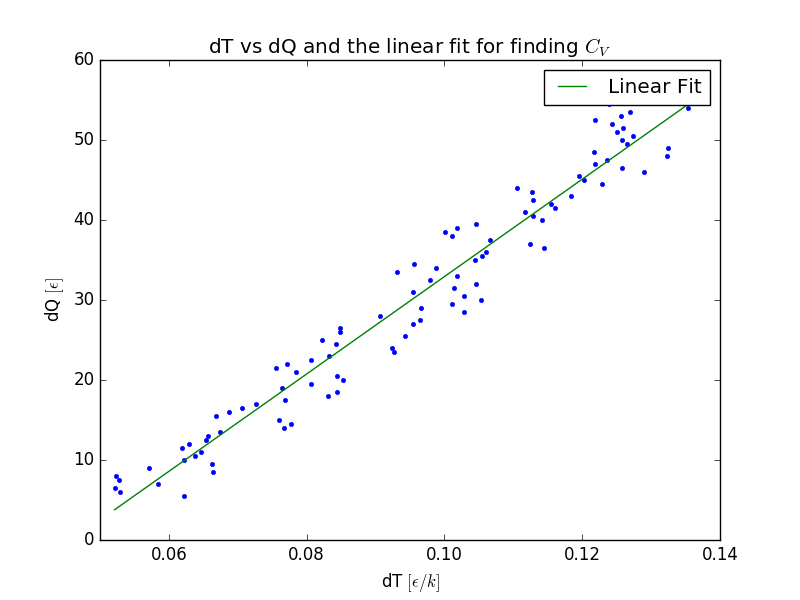
\includegraphics[scale=0.5]{project_2/problem_d}
\caption{$dQ$ versus $dT$ for a Lennard-Jones system with constant V.}
\label{fig:isoTherm}
\end{figure}

We have that 

\begin{equation}
C_V = \left(\pd{Q}{T}\right)_V \Rightarrow dQ = C_VdT
\end{equation}

The "fitted slope" is the $C_V$, which yields the following result

\begin{equation}
C_V \approx 611.5  k
\end{equation}


\subsection*{e.}
For an ideal gas the heat capacity is given as

\begin{equation}
C_V = \frac{NfR}{2}
\end{equation}
where $R$ is the gas constant, $f$ is the degree of freedom and $N$ is the number of particles. In Leonnard Jones units $R = 1$. All the particles are "point particles" and will therefore have $f = 3$. For $N = 540$ particles, we then get

\begin{equation}
C_V = \frac{540}{2} = 810k
\end{equation}

which is a bit above our result from problem \textbf{d}. This may be due to the fact that the Lennard-Jones potential is no a perfect model for an ideal gas or a "numerical error" due to a low number of particles.


\subsection*{f.}
The density was kept at $\rho = 0.01$ and the temperature was adjusted from the triple point temperature to 10 times the critical temperature (I used $T_{tp} = 0.694$ and $T_c = 1.32$ as these was the one I found at \url{http://www.sklogwiki.org/SklogWiki/index.php/Lennard-Jones_model}) in 6 steps. The resulting heat capacities was calculated for each temperature:

\begin{figure}[H]
\centering
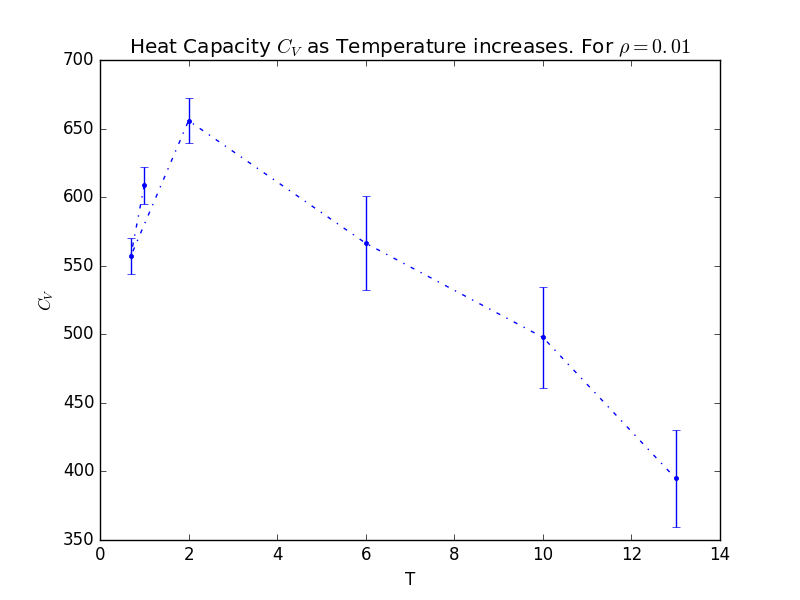
\includegraphics[scale=0.5]{project_2/problem_f}
\caption{$C_V$ as a function of temperature.}
\label{fig:isoTherm}
\end{figure}

We can see that the heat capacity seems to decrease somewhat as temperature increases. A more constant $C_V$ may have been expected\footnote{We already saw that it should be constant at $750$ k}, so the reason for this behaviour is not clear.

\subsection*{g.}

We can now do something similar to what we did above, but we instead let the temperature be constant at $T=2$, and vary the density from a diluted gas density of $\rho = 0.01$ to the triple point density of $\rho = 0.84$ (in practice I ended it at $\rho = 0.8$). We then get

\begin{figure}[H]
\centering
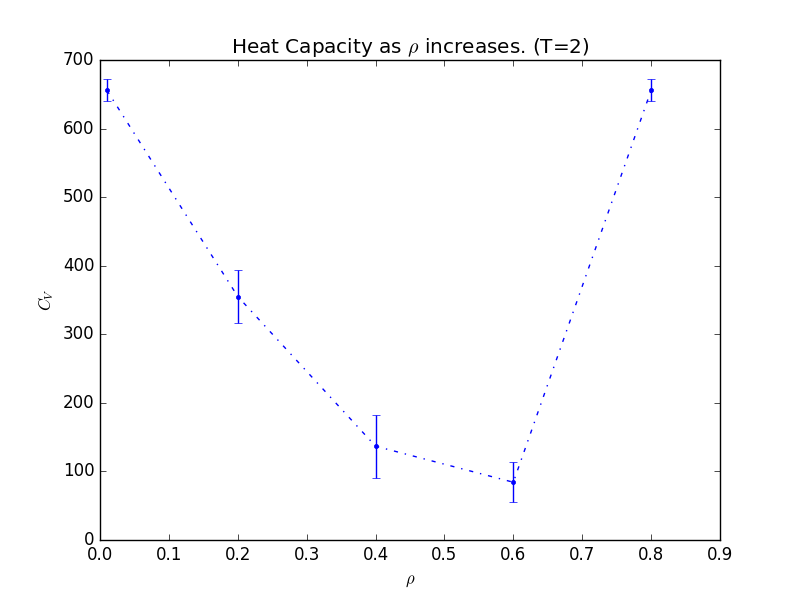
\includegraphics[scale=0.5]{project_2/problem_g}
\caption{$C_V$ as a function of density.}
\label{fig:isoTherm}
\end{figure}

Again we see a decrease in $C_V$ as $\rho$ increases. And again I am not sure why this is the case.

\subsection*{h.}
If we now hold the pressure constant we can find $C_P$. This was done with a constant temperature $T=2$ and at a diluted gas density $\rho = 0.01$ and at the triple point density.

\begin{table}[H]
\centering
\begin{tabular}{c|c|c}
& Diluted Gas & Triple Point\\
\hline
$C_V$ & 659.43 & 80.17\\
$C_P$ & 49.56 & -208.44\\
$C_P - C_P$ & -609.87 & -288.61
\end{tabular}
\caption{$C_V$ and $C_P$ at $T=2$ and for diluted gas and triple point density.}
\end{table}

We can see that both $C_P$ and $C_V$ have decreased alot from the diluted gas density to the triple point density. More important, $C_P$ should not be negative! This seems to be a problem with lammps (for me at least). At the triple point density the simulation goes its own way. Even though I use $T=2$, the simulation insist on using $T=0.92$ in the log file. The log file also gives a negative heat capacity, so it is not my calculation. Why this is, I simply don't know.

Since we need $\beta_T$ to find the theoretical value of $C_P - C_V$, which I'm not sure who to find from our simulations, since it depends on a constant temperature -- the temperature in the simulation varies. So I have nothing to compare the numerical data with, unfortunately.

\subsection*{i.}
Running the lammps script and fitting for $dQ$ vs $dT$, we get a numerical value for the heat capacity for $N_2$

\begin{equation}
C_V = 3.188
\end{equation}

We expect that the units for $C_V$ should be $[Q]/[T]$. In real unit this becomes $(Kcal/mole)/K = Kcal/(mole\cdot K)$. So

\begin{equation}
C_V = 3.188 \text{ Kcal/mole/K}
\end{equation}


\section*{Appendix}

\subsection*{Source code from project 1}

\subsubsection*{Code from problem c.}

\hypertarget{code_problem_c}{}
\lstinputlisting[language=python]{project_1/problem_c.py}


\subsubsection*{Code from problem e.}

\hypertarget{code_problem_e}{}
\lstinputlisting[language=python]{project_1/problem_e.py}


\subsubsection*{Code from problem h.}

\hypertarget{code_problem_h}{}
\lstinputlisting[language=python]{project_1/problem_h.py}


\subsubsection*{Code from problem i.}

\hypertarget{code_problem_i}{}
\lstinputlisting[language=python]{project_1/problem_i.py}


\subsection*{Source code from project 2}

\subsubsection*{Code from problem d.}

\hypertarget{code_problem_d}{}
\lstinputlisting[language=python]{project_2/problem_d.py}


\hypertarget{code_problem_f}{}
\lstinputlisting[language=python]{project_2/problem_f.py}


\hypertarget{code_problem_g}{}
\lstinputlisting[language=python]{project_2/problem_g.py}


\hypertarget{code_problem_h}{}
\lstinputlisting[language=python]{project_2/problem_h.py}


%\hypertarget{code_problem_i}{}
%\lstinputlisting[language=python]{project_2/problem_i.py}



\

\bigskip
\bigskip
\bigskip
\bigskip

\begin{center}
Bazzinga!
\end{center}

\end{document}
